%%%% Better Poster latex template example v1.0 (2019/04/04)
%%%% GNU General Public License v3.0
%%%% Rafael Bailo
%%%% https://github.com/rafaelbailo/betterposter-latex-template
%%%% 
%%%% Original design from Mike Morrison
%%%% https://twitter.com/mikemorrison

\documentclass[a0paper,fleqn]{betterposter}

%% Set up color palettes %%%%%%%%%%%%%%%%%%%%%%%%%%%%%%%%%%%%%%%%%%%%
% Color palette GreenOrange_6 from
% https://jiffyclub.github.io/palettable/tableau/
\definecolor{pgreen}     {RGB}{50,162,81}
\definecolor{porange}    {RGB}{255,127,15}
\definecolor{pblue}      {RGB}{60,183,204}
\definecolor{pyellow}    {RGB}{255,217,74}
\definecolor{pteal}      {RGB}{57,115,124}
\definecolor{pauburn}    {RGB}{184,90,13}
%%%%%%%%%%%%%%%%%%%%%%%%%%%%%%%%%%%%%%%%%%%%%%%%%%%%%%%%%%%%%%%%%%%%%
\definecolor{mygray}{gray}{0.9}

\usepackage{hyperref}
\hypersetup{pdfborder={0 0 0},
            colorlinks=true,
            % colorlinks=false,
            urlcolor=porange,
            linkcolor=pauburn,
            citecolor=pteal}

\newcommand{\given}{\ensuremath{\,|\,}\xspace}
\newcommand{\pr}{\ensuremath{p}}

\newcommand{\data}{\ensuremath{D}\xspace}
\newcommand{\model}[1][]{\ensuremath{M_{#1}}\xspace}
\newcommand{\parameters}[1][]{\ensuremath{\Theta_{#1}}\xspace}
\newcommand{\parameter}[1][]{\ensuremath{\theta_{#1}}\xspace}
\newcommand{\diff}[1]{\ensuremath{\mathrm{d}#1}}

\newcommand{\distgamma}{\ensuremath{\textrm{Gamma}}\xspace}
\newcommand{\distexponential}{\ensuremath{\textrm{Exponential}}\xspace}
\newcommand{\distbeta}{\ensuremath{\textrm{Beta}}\xspace}
\newcommand{\dgamma}[2]{\ensuremath{\distgamma(\textrm{shape} = #1, \textrm{mean} = #2)}}
\newcommand{\dexponential}[1]{\ensuremath{\distexponential(\textrm{mean} = #1)}}
\newcommand{\dbeta}[2]{\ensuremath{\distbeta(\alpha = #1, \beta = #2)}}

\newcommand{\ncomparisons}{\ensuremath{\mathcal{N}}\xspace}
\newcommand{\nevents}[1][]{\ensuremath{k_{#1}}\xspace}
\newcommand{\nexistingcats}{\ensuremath{\mathcal{K}}\xspace}
\newcommand{\nloci}[1][]{\ensuremath{m_{#1}}\xspace}

\newcommand{\observedallelecount}[1][]{\ensuremath{n_{#1}}\xspace}
\newcommand{\observedredallelecount}[1][]{\ensuremath{r_{#1}}\xspace}

\newcommand{\nodeallelecount}[2]{\ensuremath{n_{#1}^{#2}}}
\newcommand{\noderedallelecount}[2]{\ensuremath{r_{#1}^{#2}}}

\newcommand{\allelecount}[1][]{\ensuremath{\nodeallelecount{#1}{}}\xspace}
\newcommand{\redallelecount}[1][]{\ensuremath{\noderedallelecount{#1}{}}\xspace}

\newcommand{\leafallelecounts}[1][]{\ensuremath{\mathbf{n}_{#1}}\xspace}
\newcommand{\leafredallelecounts}[1][]{\ensuremath{\mathbf{r}_{#1}}\xspace}
\newcommand{\maxleafallelecounts}{\ensuremath{\textrm{max}(\mathbf{n})}\xspace}

\newcommand{\comparisondata}[1][]{\ensuremath{D_{#1}}\xspace}
\newcommand{\alldata}[1][]{\ensuremath{\mathbf{D}}\xspace}

\newcommand{\branchindex}{\ensuremath{x}\xspace}
\newcommand{\allelecountbottom}[1][\branchindex]{\nodeallelecount{#1}{B}}
\newcommand{\allelecounttop}[1][\branchindex]{\nodeallelecount{#1}{T}}
\newcommand{\redallelecountbottom}[1][\branchindex]{\noderedallelecount{#1}{B}}
\newcommand{\redallelecounttop}[1][\branchindex]{\noderedallelecount{#1}{T}}

\newcommand{\cpp}{\upshape\texttt{C++}\xspace}
\newcommand{\ecoevolity}{\upshape\texttt{ecoevolity}\xspace}
\newcommand{\simcoevolity}{\upshape\texttt{simcoevolity}\xspace}
\newcommand{\sumcoevolity}{\upshape\texttt{sumcoevolity}\xspace}
\newcommand{\pycoevolity}{\upshape\texttt{pycoevolity}\xspace}
\newcommand{\dpprobs}{\upshape\texttt{DPprobs}\xspace}

\newcommand{\wunif}{WU\xspace}

\newcommand{\rgmurate}{\ensuremath{u}\xspace}
\newcommand{\grmurate}{\ensuremath{v}\xspace}
\newcommand{\murate}[1][]{\ensuremath{\mu_{#1}}\xspace}
\newcommand{\murates}[1][]{\ensuremath{\boldsymbol{\mu}_{#1}}\xspace}
\newcommand{\gfreq}[1][]{\ensuremath{\pi_{#1}}\xspace}
\newcommand{\gfreqs}[1][]{\ensuremath{\boldsymbol{\pi}_{#1}}\xspace}

\newcommand{\comparisonetime}[1][]{\ensuremath{t_{#1}}\xspace}
\newcommand{\comparisonetimes}[1][]{\ensuremath{\mathbf{t}_{#1}}\xspace}
\newcommand{\etime}[1][]{\ensuremath{\tau_{#1}}\xspace}
\newcommand{\etimes}[1][]{\ensuremath{\boldsymbol{\tau}_{#1}}\xspace}
\newcommand{\etimemodel}[1][]{\ensuremath{T_{#1}}\xspace}
\newcommand{\etimesets}{\ensuremath{\mathcal{T}}\xspace}
\newcommand{\genetree}[1][]{\ensuremath{g_{#1}}\xspace}
\newcommand{\sptree}[1][]{\ensuremath{S_{#1}}\xspace}
\newcommand{\sptrees}[1][]{\ensuremath{\mathbf{S}_{#1}}\xspace}

\newcommand{\descendantpopindex}[1]{\ensuremath{D{#1}}}
\newcommand{\rootpopindex}[1][]{\ensuremath{R{#1}}\xspace}
\newcommand{\epopsize}[1][]{\ensuremath{N_{e}^{#1}}\xspace}
\newcommand{\sepopsize}[1][]{\ensuremath{N}\xspace}
\newcommand{\comparisonpopsizes}[1][]{\ensuremath{\mathbb{N}_{e}{#1}}\xspace}
\newcommand{\collectionpopsizes}[1][]{\ensuremath{\mathbf{N_{e}}_{#1}}\xspace}
\newcommand{\rootrelativepopsize}{\ensuremath{R_{\epopsize[\rootpopindex]}}\xspace}

\newcommand{\dirp}{\ensuremath{\textrm{DP}}\xspace}
\newcommand{\concentration}{\ensuremath{\alpha}\xspace}
\newcommand{\discount}{\ensuremath{d}\xspace}
\newcommand{\splitweight}{\ensuremath{s}\xspace}
\newcommand{\basedistribution}{\ensuremath{H}\xspace}
\newcommand{\gshape}{\ensuremath{k}\xspace}
\newcommand{\gscale}{\ensuremath{\theta}\xspace}

\newcommand{\proposed}{\ensuremath{^{\prime}}\xspace}
\newcommand{\tuningparameter}{\ensuremath{\lambda}\xspace}
\newcommand{\uniformdeviate}{\ensuremath{u}\xspace}


\usepackage[backend=biber,style=numeric]{biblatex}
\addbibresource{../bib/references.bib}

%%%% Uncomment the following commands to customise the format

%% Setting the width of columns
% Left column
\setlength{\leftbarwidth}{0.28\paperwidth}
% Right column
\setlength{\rightbarwidth}{0.28\paperwidth}

%% Setting the column margins
% Horizontal margin
\setlength{\columnmarginvertical}{0.02\paperheight}
% Vertical margin
\setlength{\columnmarginhorizontal}{0.02\paperheight}
% Horizontal margin for the main column
\setlength{\maincolumnmarginvertical}{0.02\paperheight}
% Vertical margin for the main column
\setlength{\maincolumnmarginhorizontal}{0.02\paperheight}

%% Changing font sizes
% Text font
%\renewcommand{\fontsizestandard}{\fontsize{28}{35} \selectfont}
% Main column font
%\renewcommand{\fontsizemain}{\fontsize{28}{35} \selectfont}
% Title font
%\renewcommand{\fontsizetitle}{\fontsize{28}{35} \selectfont}
% Author font
%\renewcommand{\fontsizeauthor}{\fontsize{28}{35} \selectfont}
% Section font
%\renewcommand{\fontsizesection}{\fontsize{28}{35} \selectfont}

%% Changing font sizes for a specific text segment
% Place the text inside brackets:
% {\fontsize{28}{35} \selectfont Your text goes here}

%% Changing colours
% Background of side columns
%\renewcommand{\columnbackgroundcolor}{black}
% Font of side columns
%\renewcommand{\columnfontcolor}{gray}
% Background of main column
%\renewcommand{\maincolumnbackgroundcolor}{empirical}
%\renewcommand{\maincolumnbackgroundcolor}{theory}
%\renewcommand{\maincolumnbackgroundcolor}{methods}
%\renewcommand{\maincolumnbackgroundcolor}{intervention}
% Font of main column
%\renewcommand{\maincolumnfontcolor}{gray}

\begin{document}
\betterposter{
%%%%%%%% MAIN COLUMN

\maincolumn{
%%%% Main space

\vspace{-2.5ex}
{\raggedright
All three models perform well, PYP model performs slightly better.}

\vspace{-1.5ex}
\begin{center}
\fcolorbox{white}{white}{
\begin{minipage}[t]{0.92\textwidth}
\begin{center}
\vspace{-1.5ex}
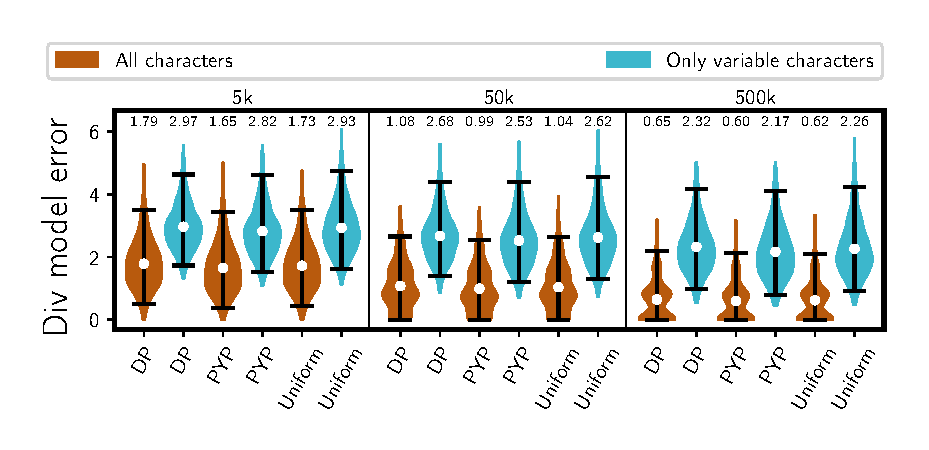
\includegraphics[width=0.92\textwidth]{../images/from-project-repo/poster-nchars-model-distance-violin-cropped.pdf}\\
\vspace{-3.3ex}
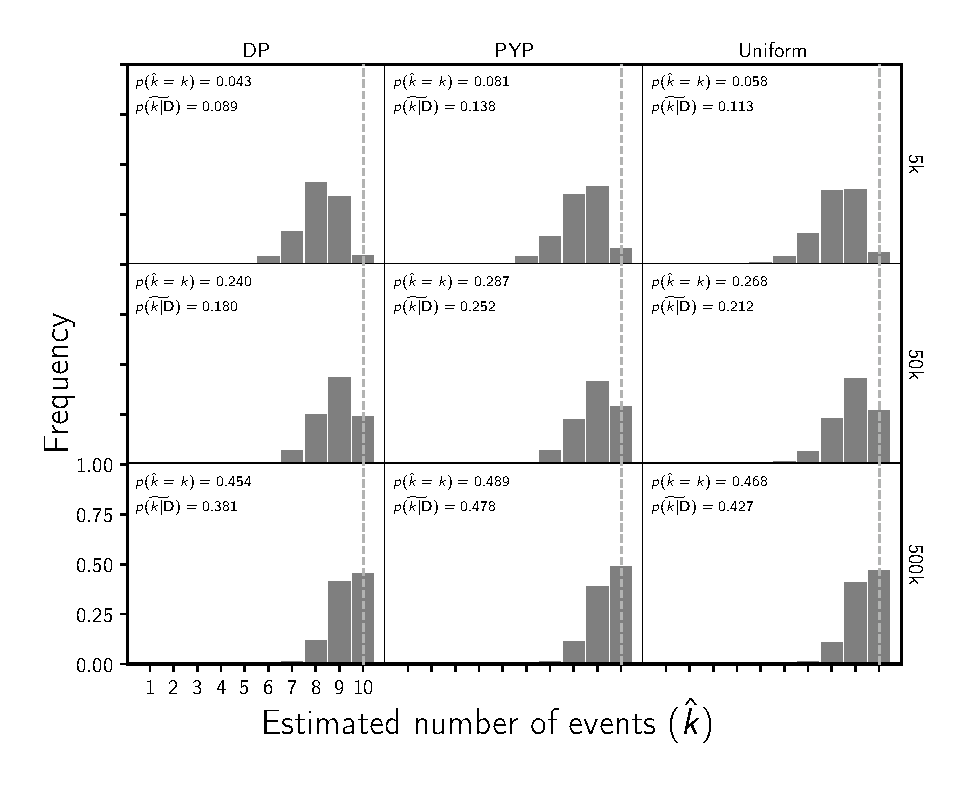
\includegraphics[width=0.92\textwidth]{../images/from-project-repo/poster-nchars-nevents-cropped.pdf}\\
\vspace{-2.5ex}
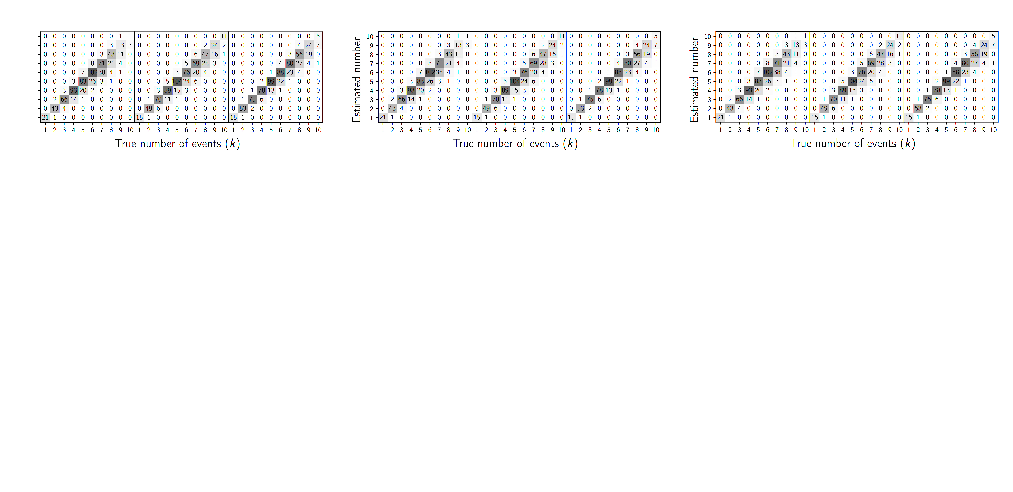
\includegraphics[width=0.92\textwidth]{../images/from-project-repo/poster-match-nevents-cropped-rasterized.pdf}
\vspace{-1.5ex}
\end{center}
\end{minipage}}
\end{center}

\vspace{-20ex}
}{
%%%% Bottom space

%% QR code
\hspace{10em}
\qrcode{../images/qr-code.png}{../images/smart-phone-white.png}{
\textbf{Take a picture} to visit
\\the \textbf{project website}
}
% \compactqrcode{../images/qr-code.png}{
% \textbf{Take a picture} to
% \\visit the project website
% }
% Smartphone icon
% Author: Freepik
% Retrieved from: https://www.flaticon.com/free-icon/smartphone_65680

%% Compact QR code (comment the previous command and uncomment this one to switch)
%\compactqrcode{img/qrcode}{
%\textbf{Take a picture} to
%\\download the full paper
%}

}

}{
%%%%%%%% LEFT COLUMN

\title{Improving estimation of shared evolutionary events}
\author{Tashitso Anamza}
\author{Jamie Oaks}
\vspace{0.5ex}
\institution{Auburn Univeristy}

\vspace{-2ex}
\section{Background}
\vspace{-0.5ex}
Environmental processes that cause speciation across communities of species
should generate patterns of divergences that are temporally clustered across
species.
\href{http://phyletica.org/ecoevolity/}{Ecoevolity}
is a tool for testing such patterns by estimating shared divergence
times among pairs of populations using genomic data and Bayesian model choice
\cite{Oaks2018ecoevolity}.

\vspace{0.5ex}
\begin{center}
\begin{minipage}[t]{0.6\linewidth}
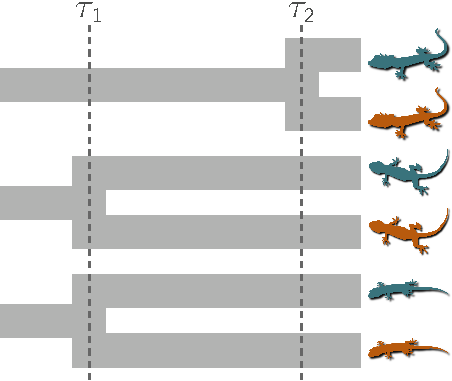
\includegraphics[width=0.9\linewidth]{../images/from-ecoevolity-tikz-repo/div-model-311-labels.pdf}\\
{\fontsize{28}{35} \selectfont %
An example of a shared divergence between 2 of 3 pairs of lizard populations.}
\end{minipage}
\end{center}

\vspace{1.5ex}
The number of ways the population pairs can share divergence times (i.e., the
number of divergence models) gets large as the number of species being compared
increases\cite{Bell1934}, so \textbf{we need flexible and efficient ways of assigning
    probabilities to all of them}.

\vspace{1.5ex}
\textbf{We implemented and compared 3 ways to assign prior probabilities to divergence
models}:
\vspace{1ex}
\begin{description}
    \item[Dirichlet process (DP)---] Commonly used in Bayesian statistics
        for clustering random variables. The process is controlled by a
        concentration parameter \cite{Ferguson1973, Antoniak1974}.
    \item[Pitman-Yor process (PYP)---] A generalization of the DP.  It adds
        a discount parameter that provides flexibility over the tail behavior
        of the process \cite{PitmanYor1997}.
    \item[Uniform prior---] In its simplest form, all divergence models are
        equally probable. However, we added a ``split-weight'' parameter to
        favor more or fewer divergence times; the prior probabilities of models
        with the same number of divergence times are always equal.
\end{description}


%% This fills the space between the content and the logo
\vfill

%% Institution logo
% \begin{center}
% 
\includegraphics[height=16ex]{../images/auburn-phylo-mtan-2014-orange.pdf}\\
% \end{center}

}{
%%%%%%%% RIGHT COLUMN

\vspace{-4ex}
\section{Methods}
To compare the \textbf{DP}, \textbf{PYP}, and \textbf{uniform} priors on
divergence models, we:
\begin{itemize}
\item Simulated 720 datasets of 500k biallelic characters from 10 pairs of
    populations under the \textbf{DP}, \textbf{PYP}, and \textbf{uniform}
    priors.
\item Simulated 720 datasets of 5k, 50k, and 500k characters under a model
    where the 10 pairs of populations all \textbf{diverge independently};
    their divergence times are drawn from an exponential distribution with a
    mean of 0.05 subsitutions per site.
    \textbf{This is the most challenging divergence model to estimate}.
\item Analyzed each of these datasets, with and without invariant characters,
    under the \textbf{DP}, \textbf{PYP}, and \textbf{uniform} priors
    to determine which is best at estimating the correct number of divergence
    times and assignment of pairs to those times.
\end{itemize}

\vspace{-1ex}
\section{Conclusions}
All three priors on divergence models performed well.
The \textbf{PYP prior performed slightly better than the DP and uniform
    priors},
likely due to the additional flexibility provided by the discount parameter.
\textbf{All three priors performed much better when invariant characters were
included in analyses.}

\vspace{-1ex}
\section{Acknowlegdements}
We thank all the members of the
\href{http://phyletica.org}{Phyletica Lab},
and NSF for funding this work (DEB 1656004).
% The computational work was made possible by the Auburn University (AU) Hopper
% Cluster supported by the AU Office of Information Technology.
This poster is based on the
\href{https://github.com/rafaelbailo/betterposter-latex-template}{Better Poster Latex Template}
developed by
\href{https://github.com/rafaelbailo}{Rafael Bailo}

\AtNextBibliography{\Huge}
\vspace{-1ex}
\section{References}
\printbibliography[heading=none]

\vfill

\begin{center}

\includegraphics[height=16ex]{../images/auburn-phylo-mtan-2014-orange.pdf}
\hspace{2em}

\includegraphics[height=16ex]{../images/aumnh-crop.png}
\end{center}

}
\end{document}
